\subsection{Metrics}\label{subsec:metrics}
\subsubsection{Metrics definition}\label{subsubsec:metrics-definition}

In this study, the performance of five algorithms - H, S, G, RW, RS - was evaluated on the Quadratic Assignment Problem (QAP).
The choice of metrics used for comparison was carefully considered to provide a comprehensive evaluation of each algorithm's performance.

The metrics selected for evaluation are as follows:

\begin{itemize}
    \item \textbf{Running Time ($T$):} The time of execution of algorithm on a given instance.
    \item \textbf{Quality ($Q$):} The quality of the solution achieved by each algorithm, calculated using the formula:
    \[ Q = 1 - \frac{(cost - cost^{*})}{cost} \]
    where $cost$ represents the total cost of the solution and $cost^{*}$ represents the optimal cost.
    \item \textbf{Instance Efficiency ($\textit{Eff}_i$):} The efficiency of each algorithm on a given instance, calculated as:
    \[ \textit{Eff}_i = \frac{Quality}{1 + \frac{Time - \min(Time)}{\max(Time) - \min(Time)}} \]
    Here, $\min(Time)$ and $\max(Time)$ represent the minimal and maximal execution times across all algorithms being compared.
\end{itemize}


\subsubsection{Metrics justification}\label{subsubsec:metrics-justification}

The quality of the solution is crucial in determining the effectiveness of each algorithm.
To quantify how close each algorithm's solution is to the optimal solution, the quality metric, defined as $Q = 1 - \frac{(cost - cost^{*})}{cost}$, has been chosen.
This metric allows for a direct comparison of the solution quality across different algorithms.
It is normalized to the range $[0, 1]$,
where $Q = 1$ indicates an optimal solution and as $Q$ approaches $0$, the solution quality decreases.
This property makes it suitable for comparing the performance of different algorithms on the same instances.

The instance efficiency metric offers a comprehensive measure of algorithm performance by incorporating both solution quality and running time.
This metric accounts for variations in solution quality and running time across different instances, allowing for fair comparisons among algorithms.
By normalizing the quality of solutions with respect to the range of execution times,
it provides a balanced assessment that considers the trade-offs between solution optimality and computational efficiency.
Furthermore, the instance efficiency metric facilitates comparisons across multiple algorithms by standardizing the evaluation process.
It enables to gauge the relative effectiveness of different algorithms in solving the same set of instances,
irrespective of their inherent complexities or computational requirements.
However, it's important to note that the instance efficiency metric may not accurately capture the difficulty of individual instances,
as the range of running times can vary significantly.
Therefore, while it serves as a useful tool for comparing algorithm performance across different instances,
it may not fully reflect the intricacies of specific problem instances.

Overall, the instance efficiency metric provides a valuable framework for assessing algorithmic performance in a comprehensive and standardized manner,
aiding in making informed decisions about algorithm selection and optimization strategies.


\subsection{Results}\label{subsec:results}
The experimental results are depicted in~\ref{fig:1}.
It is evident that subsequent instances become increasingly challenging, resulting in a decrease in solution quality for most algorithms.
An exception is observed with the Heuristic algorithm, which manages to maintain consistent solution quality across all instances.
However, it's worth noting that solutions produced by the Heuristic algorithm are inferior to those of other algorithms for all instances except one (chr18a),
where the Random Walk algorithm yields a slightly worse solution.
The advantage of the Heuristic algorithm lies in its superior speed compared to other algorithms.
This advantage is reflected in the efficiency metric, where the Heuristic algorithm outperforms random algorithms on instances chr12a and chr15a,
and emerges as the best-performing algorithm on the remaining two instances.
This can be attributed to the deterministic nature of the Heuristic algorithm, which avoids the complexities associated with extensive space exploration.


The Steepest and Greedy Algorithms yield the best results,
with the Steepest algorithm slightly outperforming the Greedy algorithm in terms of both solution quality and efficiency for the first two instances.
Conversely, the Greedy algorithm demonstrates a slight advantage over the Steepest algorithm for the last two instances.
One notable distinction between these algorithms is their approach to non-improving moves: the Steepest algorithm allows for a certain number of such moves,
whereas the Greedy algorithm terminates when no further improvement is possible.
This suggests that, for less challenging instances, permitting non-improving moves could be beneficial.
Although there is a difference between these two algorithms, it is not significant,
and the choice between them should be based on the specific requirements of the problem.
Moreover, the running time is practically identical for both algorithms.

On the other hand, the Random Walk and Random Search algorithms yield poor results.
While the quality of solutions decreases with the increasing difficulty of instances,
the decline is not as pronounced as with local search algorithms (Greedy and Steepest).
The running time of these algorithms was manually constrained to match the execution time of the Greedy and Steepest algorithms.


\begin{figure}[H]
    \centering
    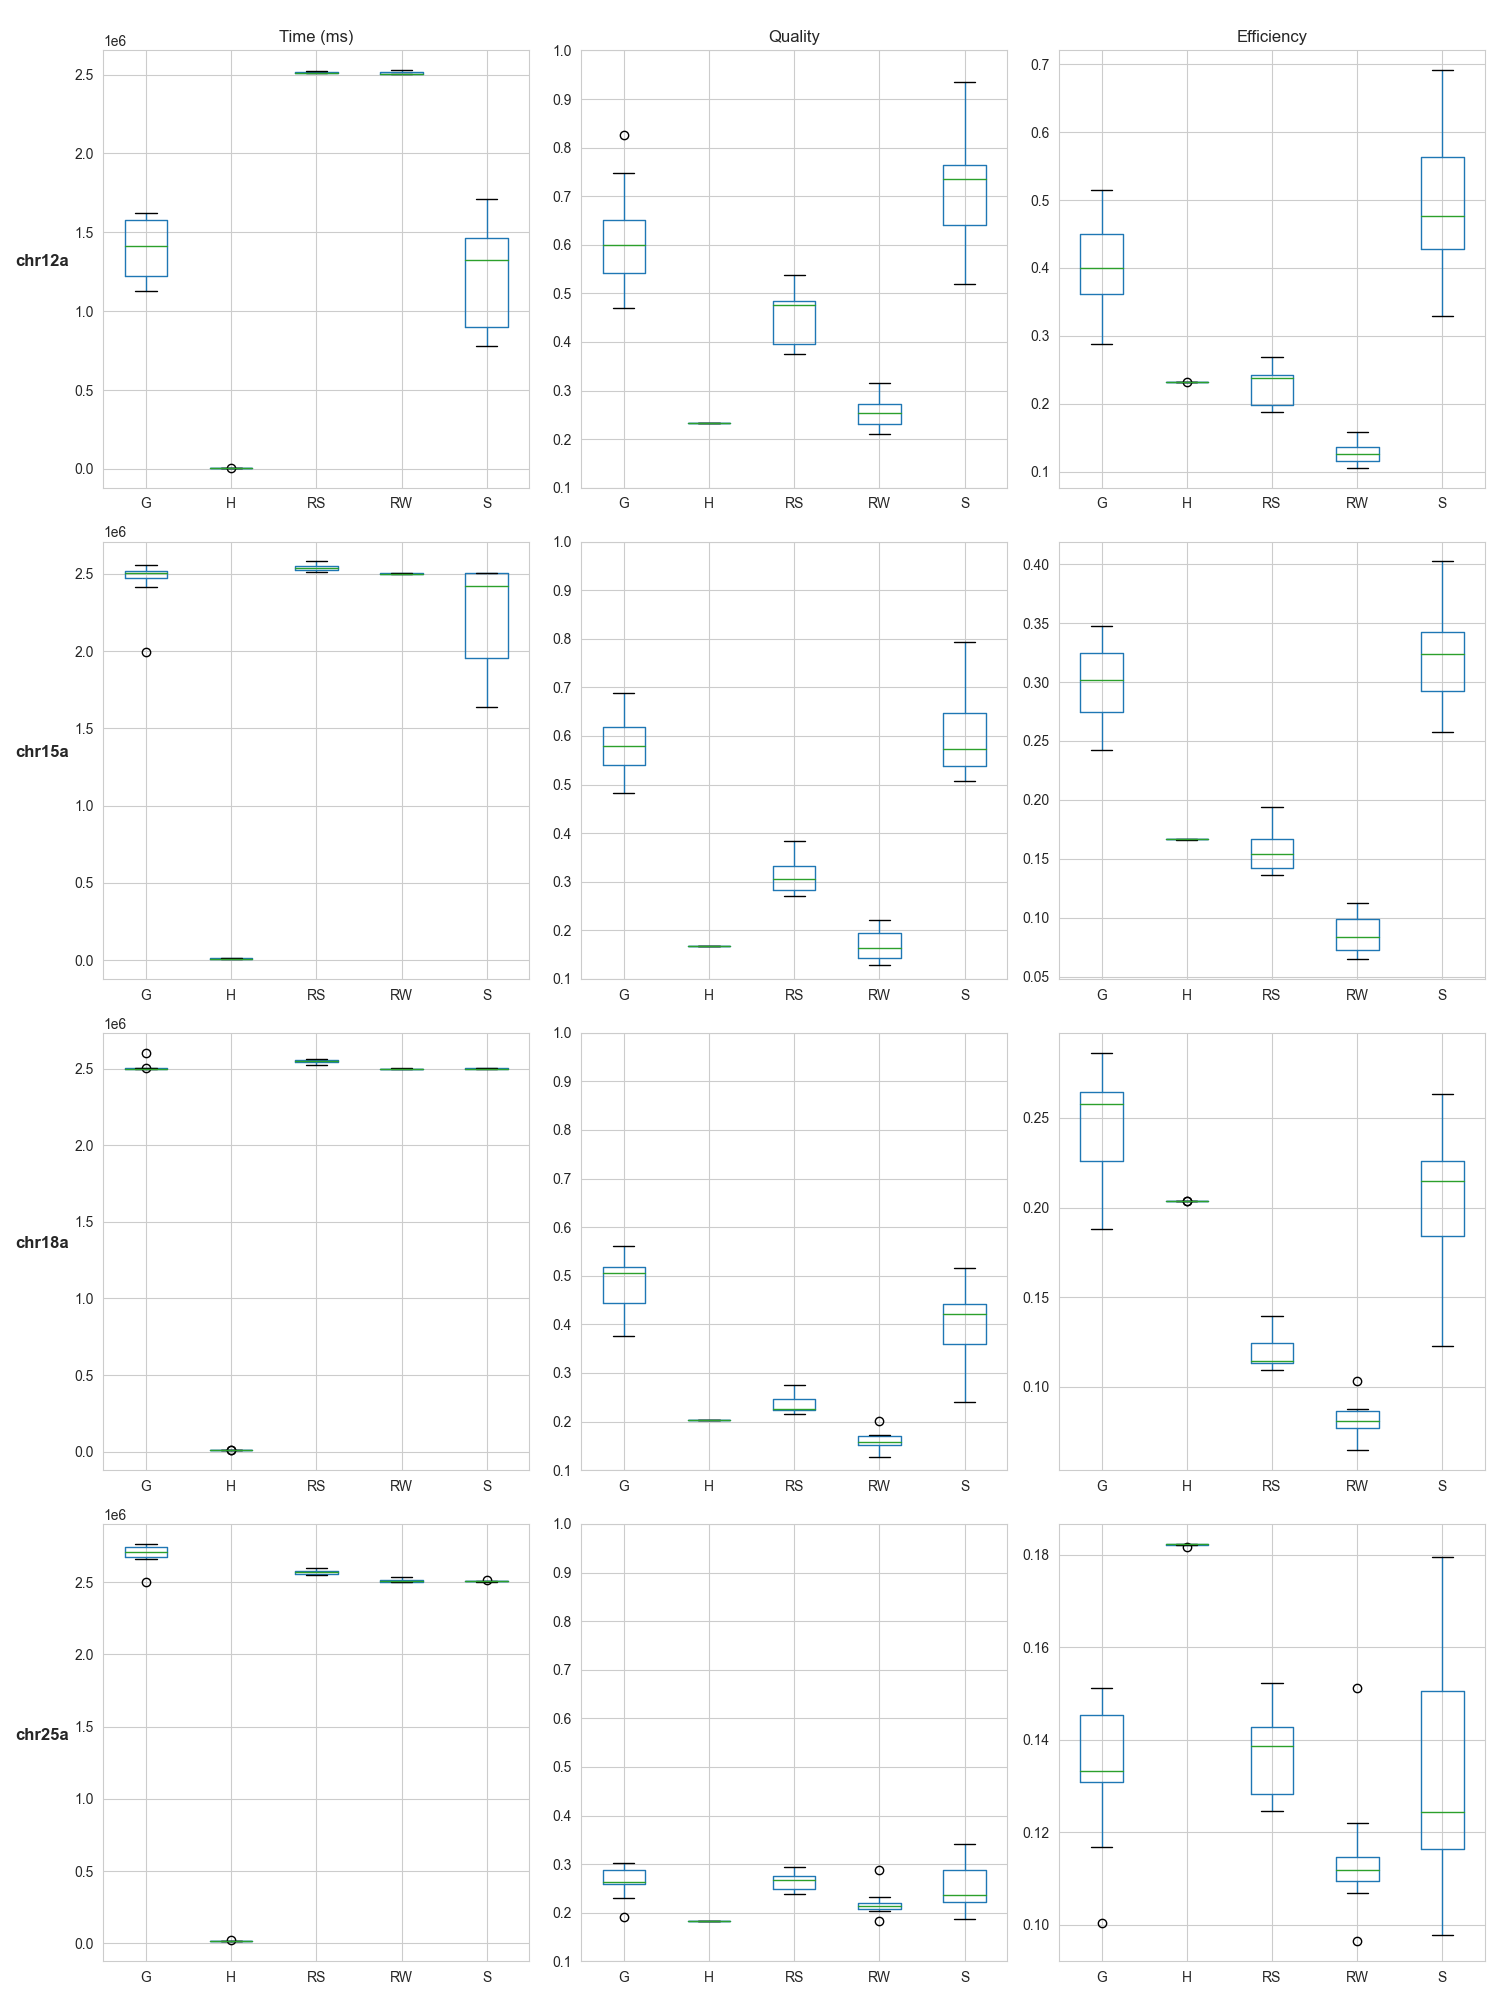
\includegraphics[width=1.0\textwidth]{pics/time_quality_efficiency_box_plots}
    \caption{Comparison of algorithms performance}
    \label{fig:1}
\end{figure}

\pagebreak

In Figure~\ref{fig:2}, the number of algorithmic steps (changes to the current solution) is depicted on the right side of the plot,
while the number of evaluated (fully or partially) solutions is shown on the left side.
The number of algorithmic steps is higher for the Greedy Algorithm compared to the Steepest Algorithm.
This disparity arises because the Greedy Algorithm continuously modifies the solution to maximize improvement,
while the Steepest Algorithm evaluates all possible neighbors before selecting the best one, resulting in less frequent solution changes.
Conversely, the number of evaluated solutions is lowest for the Random Search algorithm.
This is because Random Search requires full evaluation of each solution to assess its quality, which is more time-consuming compared to partial evaluation.
Additionally, there is a cost associated with updating the best encountered solution,
which requires copying the entire solution—a process that is not necessary for algorithms like Greedy and Steepest, where only two elements are swapped.

The Greedy algorithm conducts fewer evaluations than the Steepest and Random Walk algorithms because it does not allow for non-improving moves
and can terminate earlier.
On the other hand, Random Walk and Steepest algorithms perform a similar number of evaluations
since they allow for non-improving moves and conduct partial evaluations at each step.


\begin{figure}[H]
    \centering
    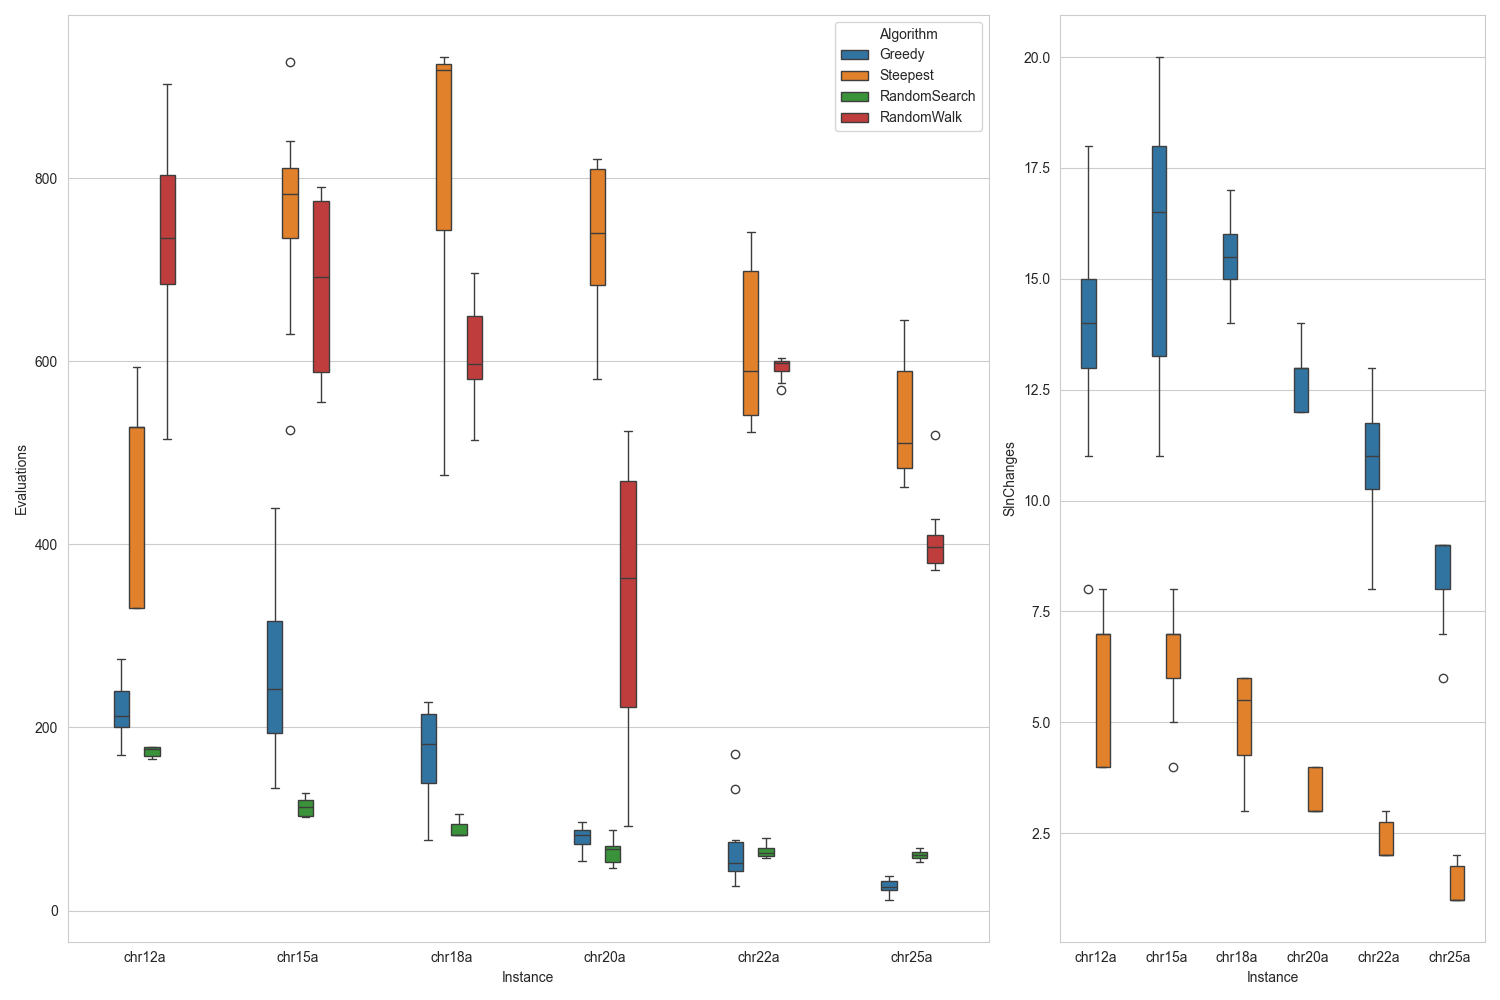
\includegraphics[width=1.0\textwidth]{pics/evaluations_sln_changes_box_plot}
    \caption{Number of algorithmic steps and evaluated solutions}
    \label{fig:2}
\end{figure}

\subsection{Initial solution influence}\label{subsec:initial-solution-influence2}
Figure~\ref{fig:3} illustrates the relationship between the quality of the solution and the quality of the initial solution.
The test was conducted for the Greedy and Steepest algorithms across three instances: chr12a, chr20a, and lipa20a.
Interestingly, the quality of the solution does not appear to depend on the quality of the initial solution.
This observation is consistent across both algorithms and all instances, as evidenced by the correlation coefficient, which is close to zero.


\begin{figure}[H]
    \centering
    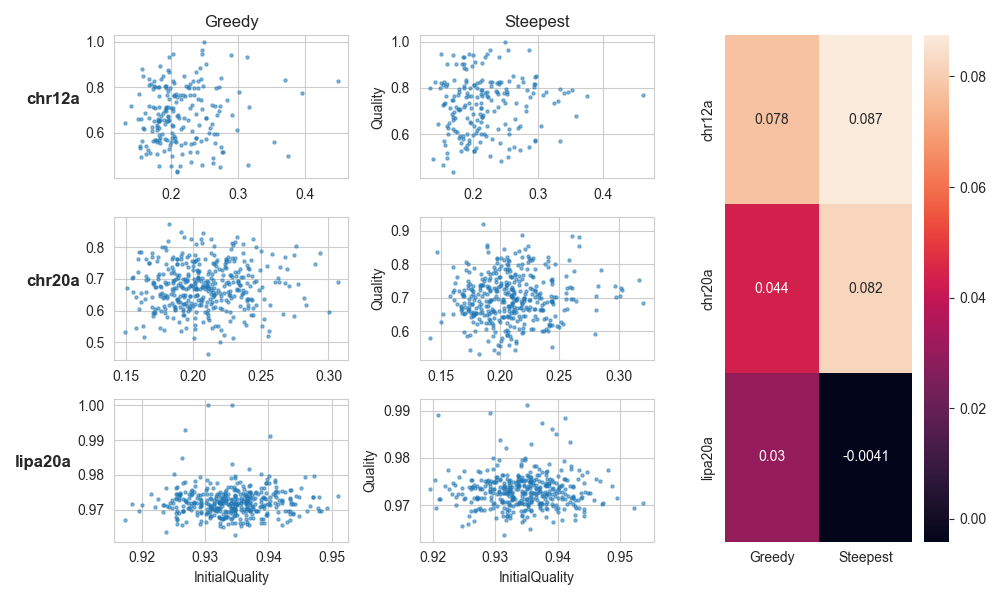
\includegraphics[width=1.0\textwidth]{pics/initial_quality_correlation_heatmap}
    \caption{Quality of the solution vs quality of the initial solution}
    \label{fig:3}
\end{figure}

\subsection{Algorithm performance over subsequent runs}\label{subsec:algorithm-performance-over-subsequent-runs}
Figure~\ref{fig:4} presents the average and lowest cost of the solution for the Greedy and Steepest algorithms obtained up to the $i$-th run.
It is noticeable that the average cost of the solution remains relatively stable after the first 50 runs.
The most significant decrease in cost occurs within the initial 10 runs.
Subsequent reductions in cost occur intermittently, with noticeable decreases observed after approximately 100 to 300 runs, depending on the instance.
Therefore, it is advisable to run the algorithm for at least 10 or 20 iterations to observe substantial improvements in solution quality.

\begin{figure}[H]
    \centering
    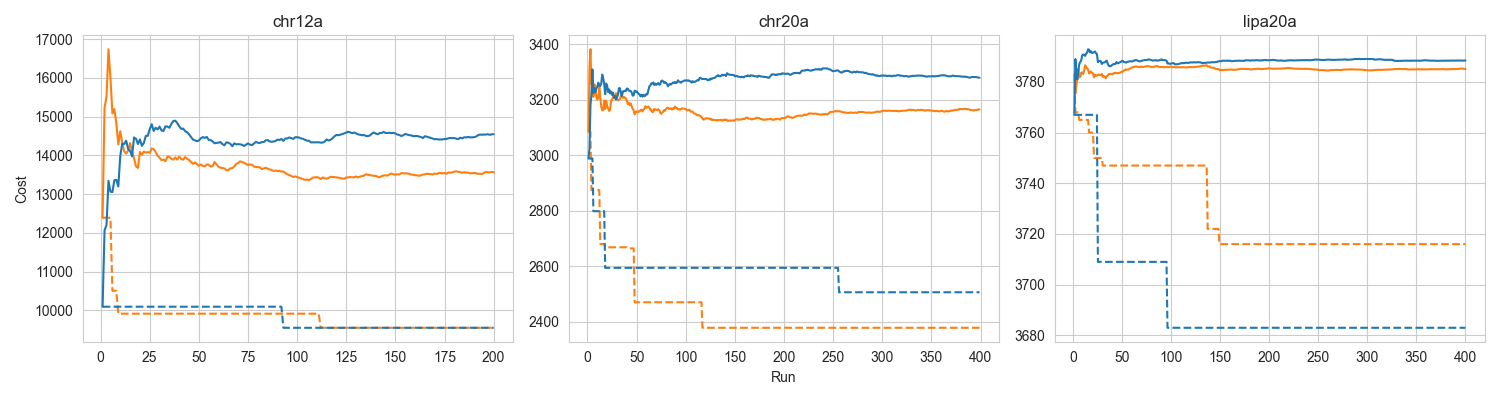
\includegraphics[width=1.0\textwidth]{pics/initial_quality_cost_so_far}
    \caption{Average and lowest cost of the solution}
    \label{fig:4}
\end{figure}

\subsection{Distance from optimal solution in decision space}\label{subsec:distance-from-optimal-solution-in-decision-space}
The correlation between the quality of the solution and the distance in decision space from the optimal solution,
calculated as the number of elements that differ between the permutation representing the solution and the optimal permutation,
is depicted in Table~\ref{tab:1} for two instances, tai12b and tai100b.
Corresponding scatter plots are provided in Figure~\ref{fig:5}.
For both instances, tai12b and tai100b, the correlation is negative,
indicating that the quality of the solution tends to decrease as the distance from the optimal solution increases.
However, the correlation is not significant, suggesting that local minima are distributed across the decision space.

\begin{table}[H]
    \centering
    \begin{tabular}{|c|c|c|}
        \hline
        Instance & Algorithm & Correlation \\
        \hline
        tai12b & Greedy & -0.46 \\
        tai12b & Steepest & -0.51 \\
        tai100b & Greedy & -0.63 \\
        tai100b & Steepest & -0.53 \\
        \hline
    \end{tabular}
    \caption{Correlation between the quality of the solution and the distance in decision space from optimal solution}
    \label{tab:1}
\end{table}

\begin{figure}[H]
    \centering
    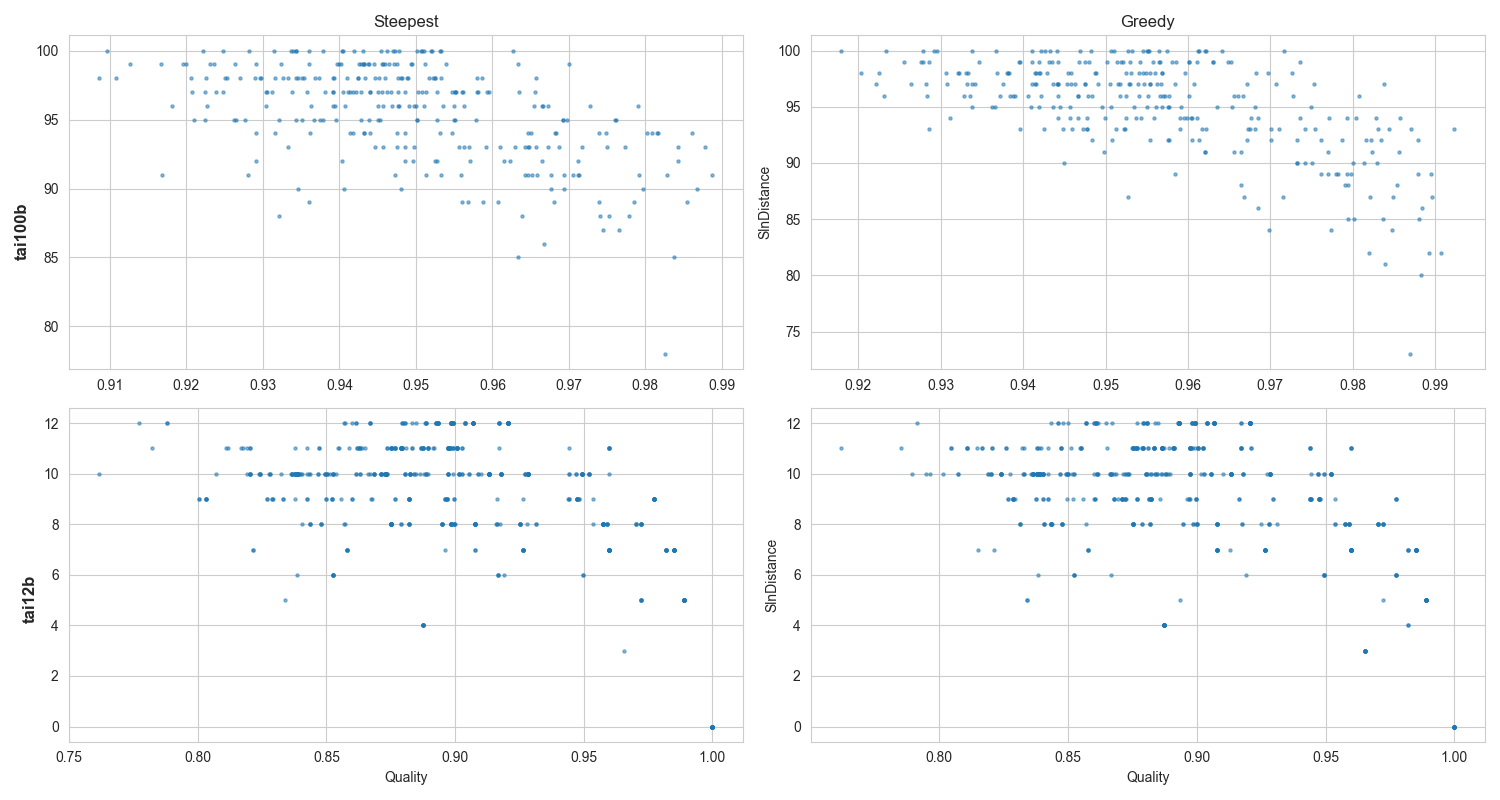
\includegraphics[width=1.0\textwidth]{pics/repetitions_quality_distance_scatter}
    \caption{Quality of the solution vs distance from optimal solution}
    \label{fig:5}
\end{figure}